\newpage
\thispagestyle{empty}
\mbox{}

\chapter{Conclusion}
\section{Introduction}
This chapter includes a discussion of the work done, the techniques employed to achieve the intended outcomes, and several constructive suggestions to enhance the quality of the thesis.

\section{The Work Process}

\subsection{Meetings}
The team held meetings with their supervisor, Filip Holik, every week. Although the meetings were typically scheduled for Wednesdays, they had to be postponed or canceled on occasions due to various circumstances. Meeting Minutes with the supervisor can be found in Appendix \ref{supervisormeeting}.
\\~\\
During the early stages of the project, the team met with the stakeholder every other week. However, as the project progressed, both parties agreed that weekly meetings would be beneficial. In addition, as the demand for help grew, the group required more regular assistance. Meeting Minutes with the stakeholder can be found in Appendix \ref{nbimmeeting}.  

\subsection{Scrum}
Throughout the thesis, the group followed the Scrum framework of agile project management, which required breaking the project into sprints lasting two to four weeks. Daily stand-up meetings were held to keep everyone informed, during which members delivered progress reports on the thesis and discussed plans for the day, including each member's allocated chores. While the group aimed to meet daily, this was sometimes difficult to achieve as some members had work obligations besides their studies.
\\~\\
Despite this, the team had sprint planning and retrospective sessions every two weeks to review progress and establish goals for the next two weeks. During the retrospective meetings, the team engaged in self-reflection by asking questions such as \say{What should we keep/stop doing?}, \say{What should we do more/less of?} to identify improvement areas for the next sprint cycle. During the sprint planning meetings, on the other hand, the group evaluated completed tasks and discussed what needed to be done before the next sprint period.
\\~\\
Following the Scrum framework helped promote good communication and teamwork among group members. Furthermore, the Kanban board was integrated into the Scrum Framework and proved to be quite helpful in tracking tasks that were ongoing, completed, or yet to be started. 

\subsection{Coordinated schedule}
In order to better coordinate their busy schedules, group members with different commitments, such as work and student associations, decided to implement a scheduling method. Doing this allowed them to quickly determine each other's availability and schedule meetings more efficiently. To achieve this, the team utilized the calendar feature within their Teams channel to schedule their activities and workdays.

\subsection{Draft Submissions}
The team set specified deadlines for producing multiple drafts at the start of the project. This approach tried to maintain constant development while avoiding last-minute delays. For instance, the group set an April 3rd target for their first draft, which they could meet. As a result, both the supervisor and the stakeholder received the first draft on time. After a few days, the team got feedback and proceeded with their work accordingly. 
\\
Additionally, the group established a deadline for the final draft. Setting the final draft deadline on the 1st of May, three weeks before the submission date of the 22nd of May, gave the stakeholders and supervisor sufficient time to review the thesis thoroughly. It is essential to mention that the group followed the plan comprehensively, allowing them to send in multiple drafts for review and refinement before the final submission. 


\subsection{Gantt Chart}
Since the group decided to change the scope during the project period, the original Gantt chart could not be followed. 
\\~\\
The research on tools was initially considered time-consuming, but with the changes made, this activity became a minor part of the thesis than anticipated. As a result, it took less time than what was first estimated. Furthermore, the \say{Testing tools} activity was removed since the team wanted to focus less on testing tools and more on integrating testing of the various tools into the pipeline-building process. 
\\~\\           
The process of learning \acrshort{aws} and configuring the pipeline with Terraform took more extended time than initially expected.
The documentation for \acrshort{aws} and Terraform is extensive, but navigating it can be overwhelming. With so many different services and features offered by \acrshort{aws}, the group had to determine the best fit for their needs. In addition, building the pipeline required a significant amount of functionality to be in place for additional features to work correctly. 
\\~\\
However, the group followed the scheduled deadlines for the various draft submissions. Consequently, the initial draft was submitted on April 3rd in week 13, but after discussions with the supervisor (see meeting minutes in Appendix \ref{ChangeFinalDraftDateMeeting}), it was requested to be rescheduled to May 5th in week 18, resulting in additional work being accomplished within those two days.

\vspace{2mm}
\begin{figure}[H]
    \centering
    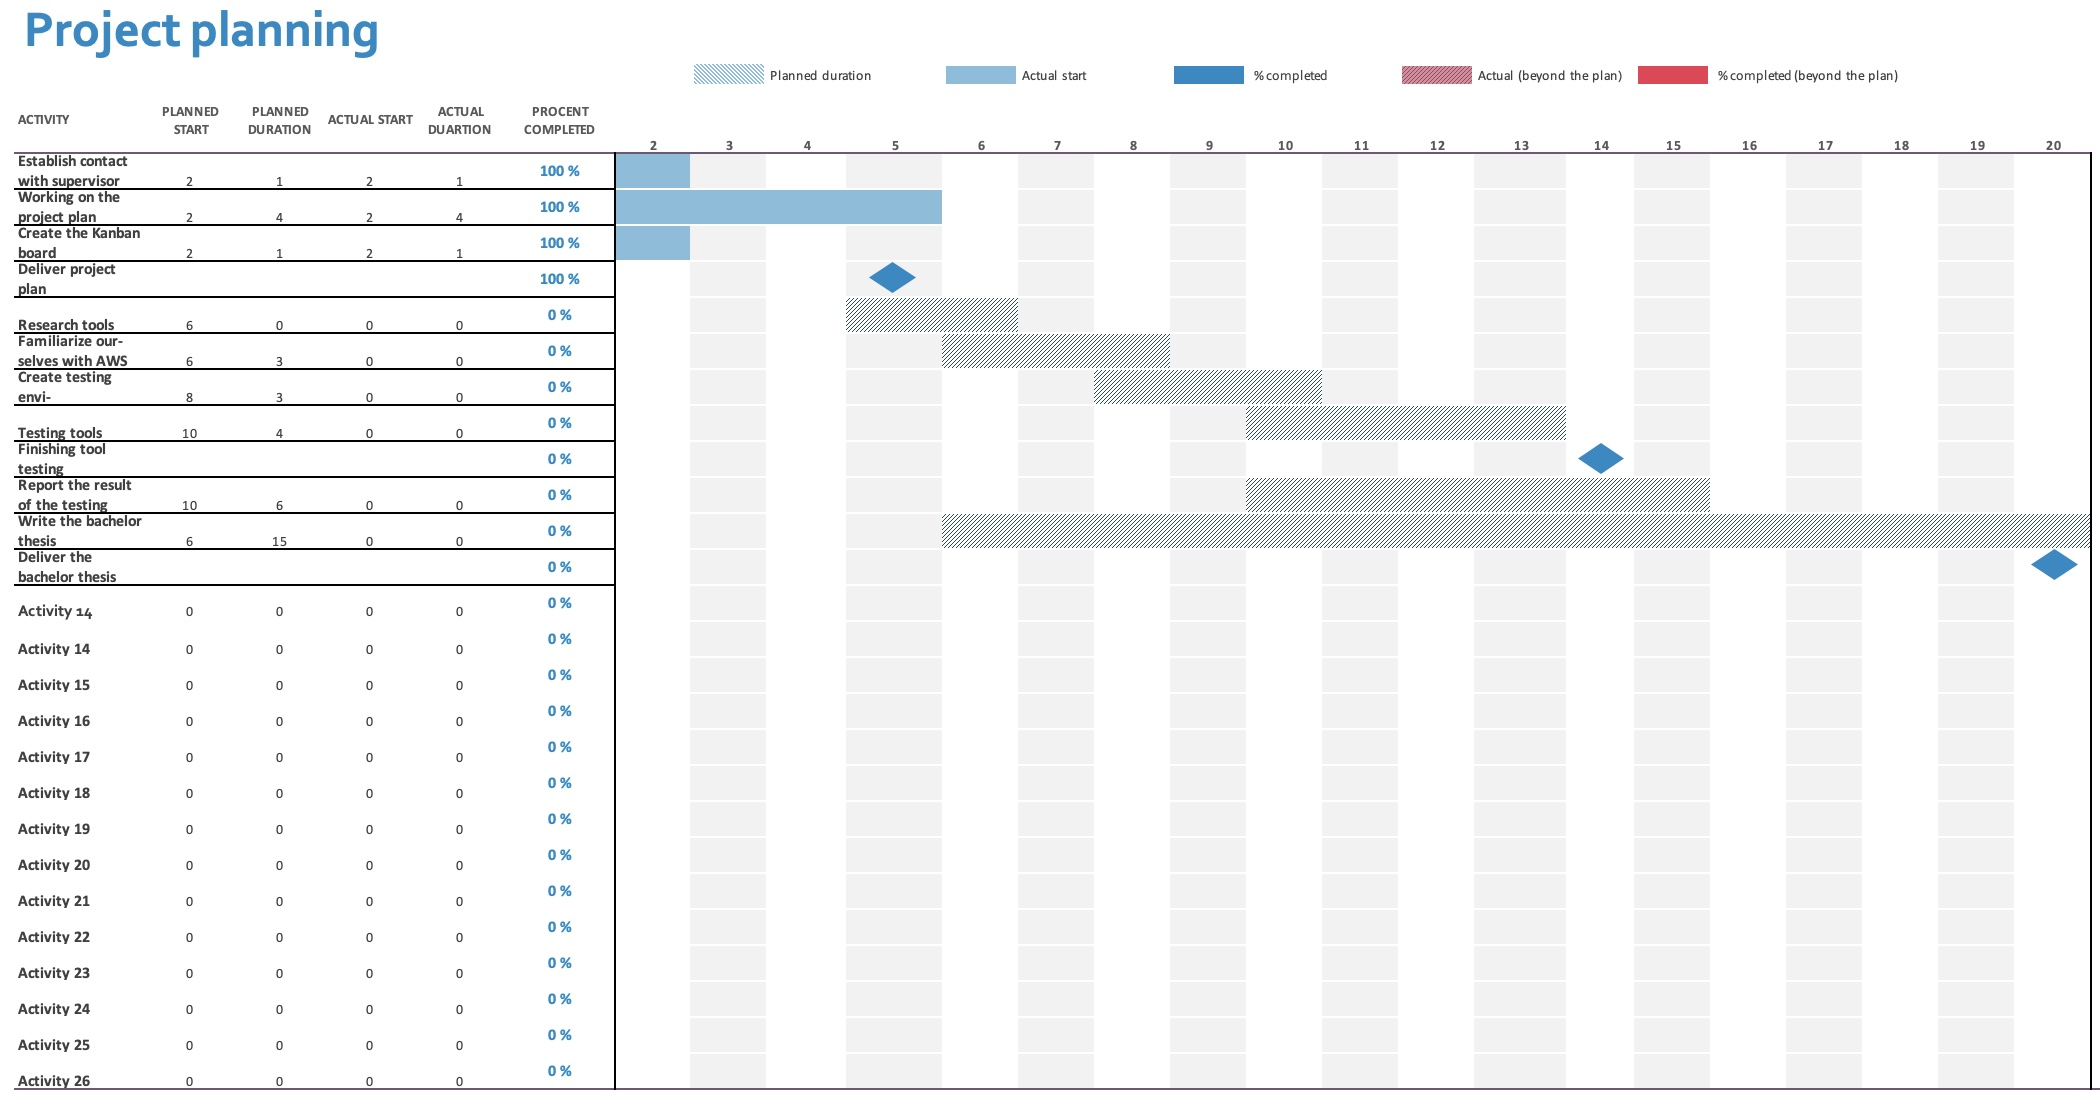
\includegraphics[width=1\columnwidth]{Images/gantt2.jpg}
    \caption{Original Gantt Chart}
    \label{fig: Original Gantt Chart}
\end{figure}

\vspace{2mm}
\begin{figure}[H]
    \centering
    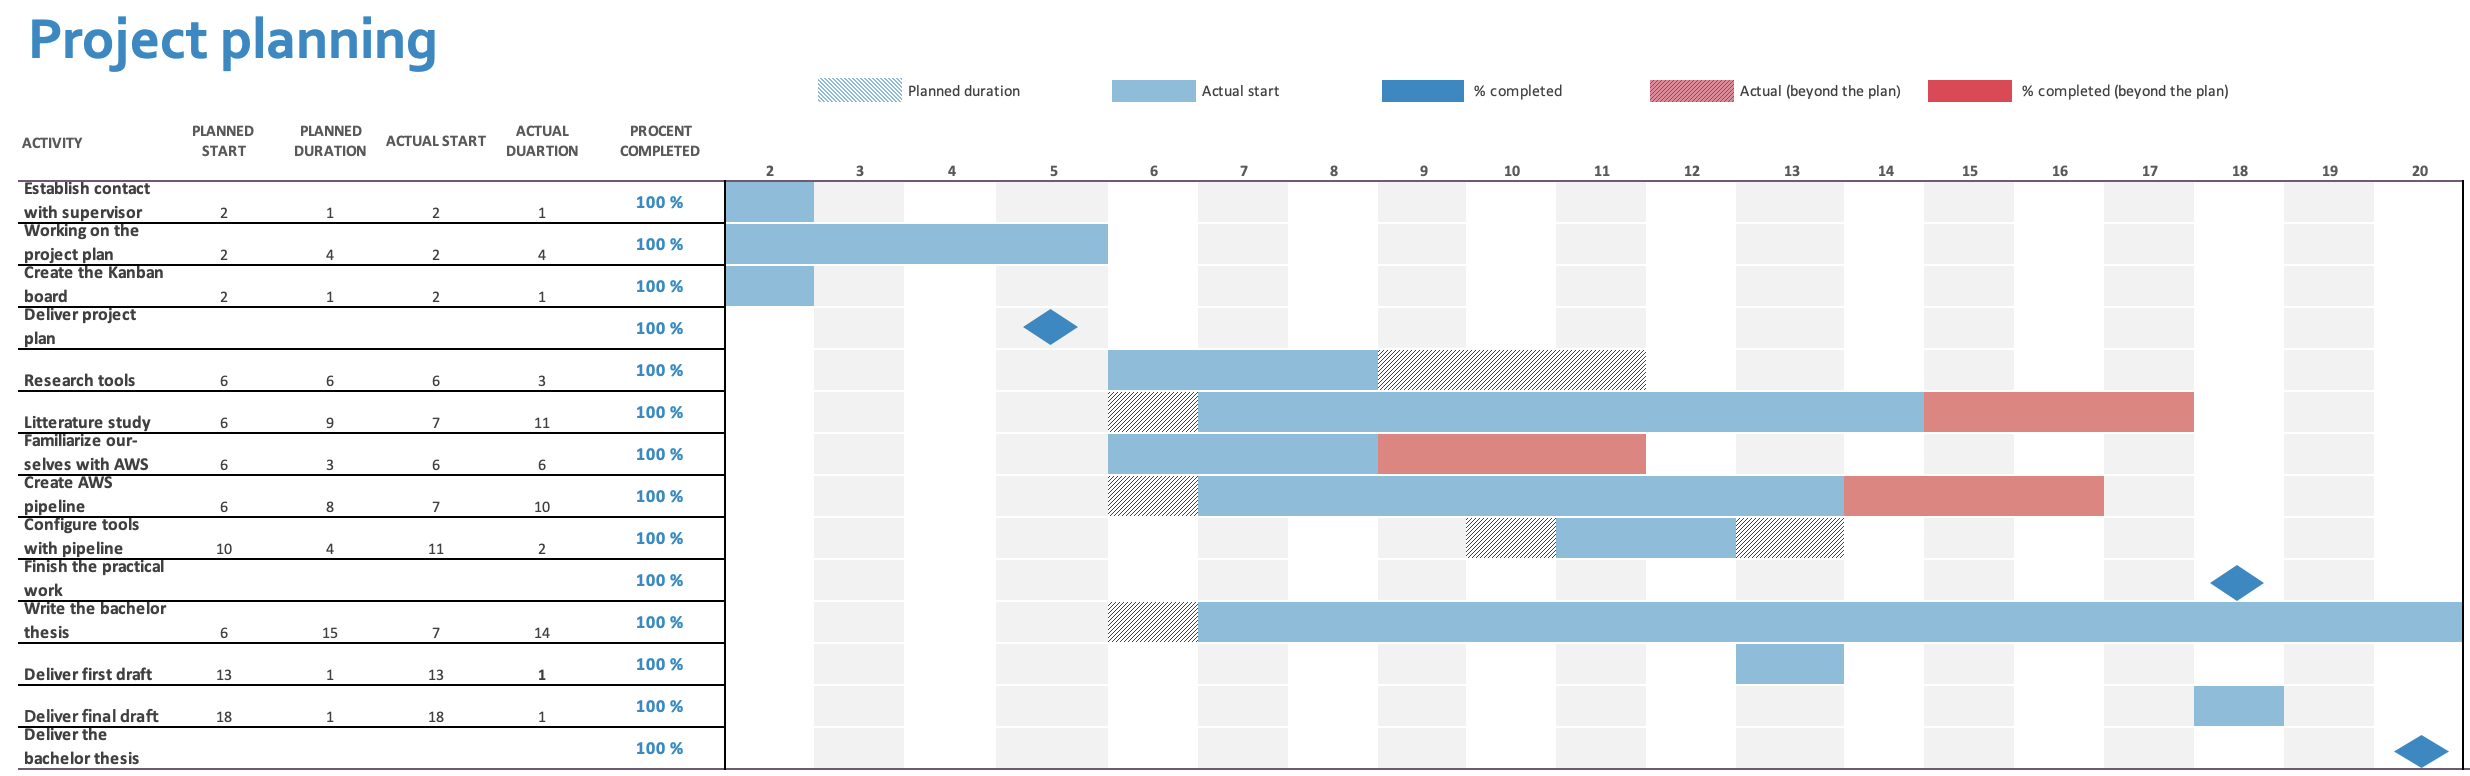
\includegraphics[width=1\columnwidth]{Images/finished-gantt.png}
    \caption{Updated Gantt Chart}
    \label{fig: Updated Gantt Chart}
\end{figure}


\subsection{Distribution of Work}
The group decided to divide the work into two parts at the start of the thesis to ensure that the thesis progressed continuously. The first part is practical, and the second is report writing. The responsibilities were assigned based on each group member's strength and what they most desired to do. As a result, every group member contributed to the thesis, and everyone worked together to complete the report on time. 

\subsection{Goals}
P1: \textit{Collaborate effectively with team members to ensure the timely completion of tasks} was achieved. As stated previously, the group incorporated a Kanban board into the Scrum framework allowing for the assignment and tracking of tasks. Additionally, the group utilized various communication platforms, such as Discord and Teams, to ensure effective communication among the group members. Using communication tools already integrated into each member's daily workflow was essential, and these two platforms proved to be the most effective for the group's needs. 
\\~\\
P2: \textit{Successfully integrating security tools (e.g., \acrshort{sast}, \acrshort{dast}, \acrshort{sca}) into the \acrshort{sdlc} \gls{pipeline}} was achieved. The group found tools that could be integrated into the \gls{pipeline} between GitHub and \acrshort{aws} to secure the application code being sent through.
\\~\\
P3: \textit{Implement an automated \gls{pipeline} using Terraform to build, test, and deploy applications} was achieved. The group created Terraform code that automated the pipeline from the build to the deployment. 
\\~\\
R1: \textit{Develop a secure and automated \gls{pipeline} for the \acrshort{sdlc} process using Terraform}, is partially achieved. The group developed an automated pipeline using Terraform code and implemented restricted access management to ensure pipeline security. However, it would be overly confident to claim that the \gls{pipeline} is 100\% secure, as the group did not have sufficient time to implement signed artifacts. This would have ensured that the code pushed to the GitHub repository was the same as the code sent through the \gls{pipeline}, thus guaranteeing code integrity. Consequently, while the \gls{pipeline} can be deemed secure, the group cannot be entirely specific that the code sent through is secure. Hence, the goal of achieving a complete, secure, and automated \gls{pipeline} remains partially fulfilled. 
\\~\\
R2: \textit{Produce a report summarizing the project results and recommendations for improving the \acrshort{sdlc} \gls{pipeline} security}, was accomplished. The resulting report provides numerous essential and effective practices that can be implemented to improve security in the \acrshort{sdlc}, and the goal was achieved within the requirements given. 

\section{Further Work}
For further work, the thesis could be strengthened by performing a broader analysis of various security tools that perform \acrshort{sast}, \acrshort{dast}, and \acrshort{sca} scans -  where the selected tools are based on these analyses. During these analyses, an assessment can also be made of which requirements must be met for a tool to be selected. 
\\~\\
Including earlier phases in the thesis would have been beneficial to acquire a more thorough grasp of the entire \acrlong{sdlc} and adhere to the shift-left methodology, which emphasizes early testing to find vulnerabilities earlier.   
\\~\\
%Despite successfully automating most of the \gls{pipeline}, the group encountered challenges in automating Secret Scanning in GitHub. The lack of documentation on enabling it through \acrshort{cli} or Terraform code limited the progress. Consequently, the group prioritized other tasks and allocated more time to this aspect in future work. The ultimate goal remains to achieve a fully automated \gls{pipeline}. 

%Write about code integrity!!!! NEED MORE OF THIS!

\section{Conclusion}
The group is pleased to state that they have completed their thesis project, meeting the requirements set by their stakeholder while staying within the project's scope. The input from the stakeholders was critical in determining the group's objectives and requirements, resulting in a successful outcome that met the expectations of everyone involved.
\\~\\
After careful consideration, the group recommends developers to implement \acrshort{sast}, \acrshort{sca} and secret scanning in the implementation phase of the \acrshort{sdlc}. Further, they recommend 



the group found that integrating Dependabot and CodeQL on GitHub was the most viable option in regards to using \acrshort{sca} and \acrshort{sast} tools. The implementation process was smooth, and the group encountered no significant issues throughout the integration. In addition, despite GitHub's lack of a \acrshort{dast} scanning option, the group could utilize \acrshort{owasp} \acrshort{zap}, which worked flawlessly with \acrshort{aws} and was easy to set up.
\\~\\
The group is confident that the stakeholder will significantly benefit from their thesis, and they highly recommend that the stakeholder consider implementing some of their recommendations in their daily work. The group is proud of their accomplishments and hopes that their work will significantly help the stakeholder.
